% 图 84.4 —— 由 `checks/emit_hand.py` 自动拼出（probe 精测 + prims2 图元分解）
%%
% ⚠ 这是**稿子不是成品**：跑 `checks/checkhand.py 84.4` 看指标 + 看叠合图。
%%
%% ⚠ 待核：
%   · 本图 probe 报出阴影族 1 个 —— **本脚本不生成阴影**（要照原书手写）；prims2 的 strokes 里可能含阴影线，核对时留意别画重
%   · 可疑字形 1 项（空心圈 ⊙ 常被认成字母 o）—— 见文件末
%%
\documentclass[12pt]{standalone}
\usepackage{fontspec}
\setsansfont{Arial}
\newfontfamily\mfallback{DejaVu Sans}
\usepackage{tikz}
\begin{document}
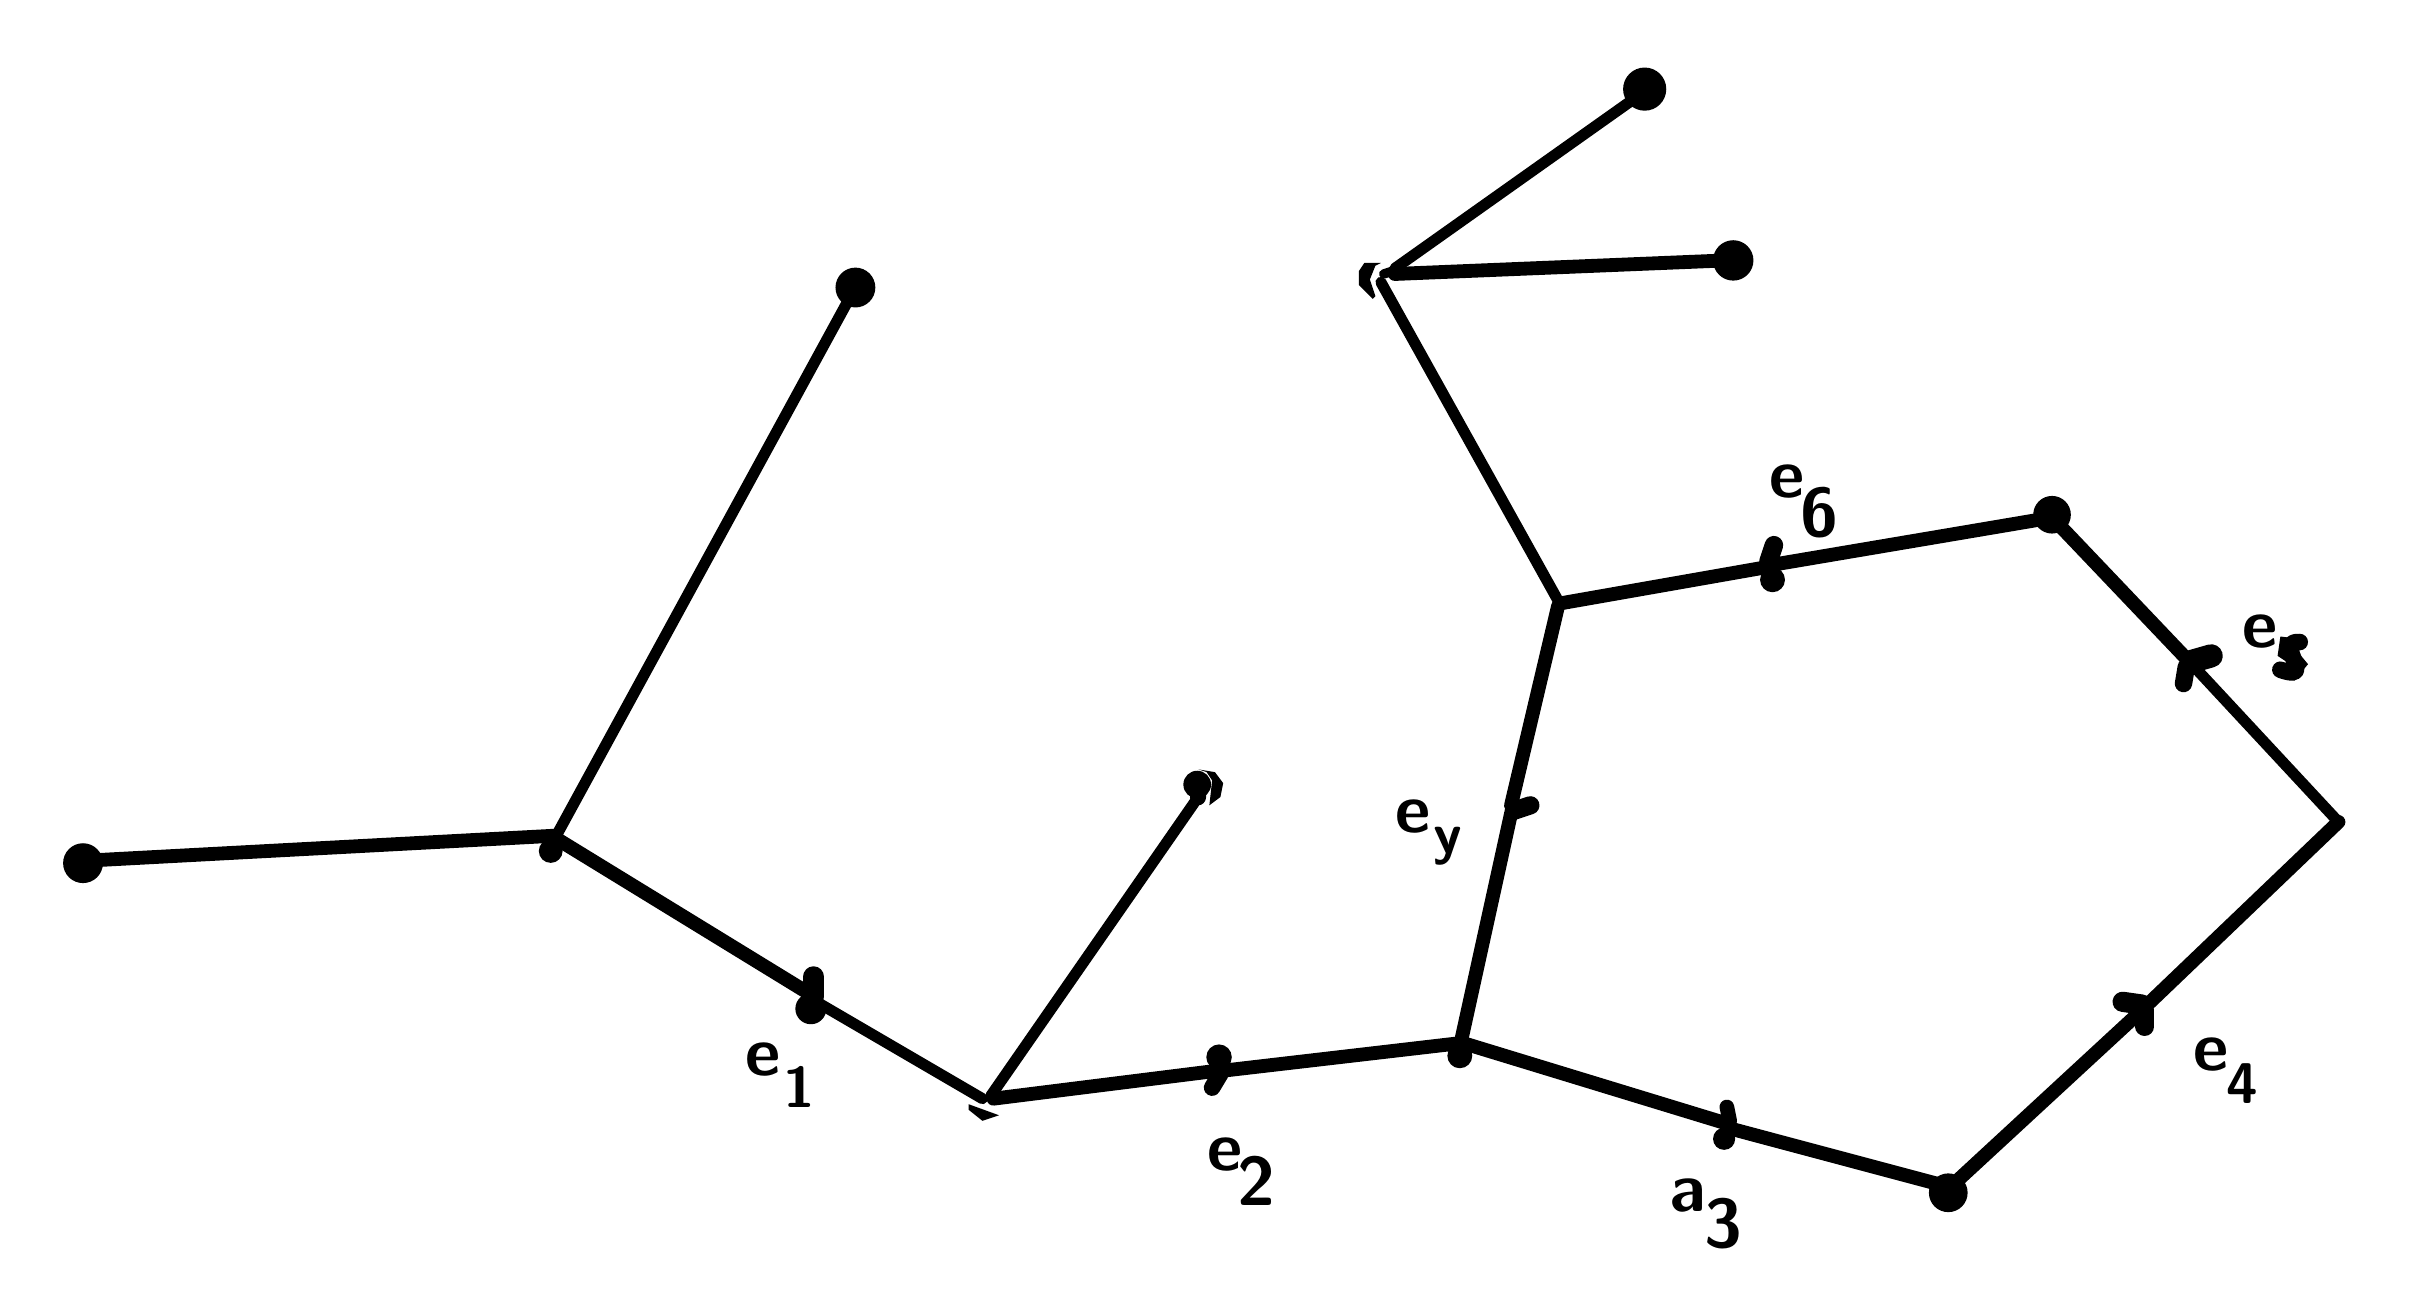
\begin{tikzpicture}[x=1pt, y=-1pt, line width=4.0pt, line cap=round, line join=round]

  %% ════ 填充区（prims2 的 fills）════
  \fill (814.0,220.0) -- (813.0,227.0) -- (819.0,231.0) -- (813.0,231.0) -- (813.0,233.0) -- (819.0,236.0) -- (824.0,230.0) -- (819.0,224.0) -- (822.0,221.0) -- cycle;
  \fill (489.0,85.0) -- (483.0,85.0) -- (481.0,88.0) -- (481.0,93.0) -- (486.0,98.0) -- (487.0,97.0) -- (485.0,91.0) -- (487.0,86.0) -- cycle;
  \fill (423.0,268.0) -- (426.0,269.0) -- (428.0,272.0) -- (427.0,281.0) -- (431.0,278.0) -- (432.0,273.0) -- (429.0,269.0) -- cycle;
  \fill (340.0,389.0) -- (340.0,391.0) -- (345.0,395.0) -- (351.0,393.0) -- cycle;

  %% ════ 直线段（prims2 的 strokes）════
  \draw[line width=4.0pt] (584.0,20.0) -- (583.3,23.7);
  \draw[line width=4.0pt] (583.3,23.7) -- (494.0,87.0);
  \draw[line width=3.4pt] (493.0,88.0) -- (490.0,89.0);
  \draw[line width=5.0pt] (628.0,195.0) -- (554.0,208.0);
  \draw[line width=7.3pt] (757.0,352.0) -- (764.0,353.0);
  \draw[line width=5.0pt] (631.0,194.0) -- (731.5,177.0);
  \draw[line width=5.0pt] (731.5,177.0) -- (781.0,229.0);
  \draw[line width=4.0pt] (345.0,387.0) -- (285.0,352.0);
  \draw[line width=6.0pt] (431.0,378.0) -- (428.0,383.0);
  \draw[line width=3.0pt] (19.0,303.0) -- (21.2,301.0);
  \draw[line width=5.0pt] (21.2,301.0) -- (190.0,292.0);
  \draw[line width=6.7pt] (765.0,361.0) -- (765.0,355.0);
  \draw[line width=7.7pt] (284.0,343.0) -- (284.0,350.0);
  \draw[line width=5.8pt] (423.0,273.0) -- (422.9,278.1);
  \draw[line width=4.0pt] (422.9,278.1) -- (348.0,386.0);
  \draw[line width=4.0pt] (782.0,230.0) -- (835.0,287.0);
  \draw[line width=6.6pt] (537.0,283.0) -- (543.0,281.0);
  \draw[line width=5.0pt] (536.0,284.0) -- (518.0,366.0);
  \draw[line width=5.0pt] (349.0,387.0) -- (429.0,377.0);
  \draw[line width=5.0pt] (284.0,350.0) -- (191.0,293.0);
  \draw[line width=5.0pt] (616.0,84.0) -- (494.0,89.0);
  \draw[line width=4.0pt] (489.0,92.0) -- (553.0,207.0);
  \draw[line width=8.4pt] (789.0,227.0) -- (782.0,229.0);
  \draw[line width=6.3pt] (780.0,231.0) -- (779.0,237.0);
  \draw[line width=4.0pt] (299.0,94.0) -- (191.0,292.0);
  \draw[line width=5.0pt] (536.0,281.0) -- (553.0,209.0);
  \draw[line width=5.0pt] (614.0,396.0) -- (519.0,367.0);
  \draw[line width=5.0pt] (517.0,367.0) -- (431.0,377.0);
  \draw[line width=5.3pt] (615.0,395.0) -- (614.0,390.0);
  \draw[line width=6.7pt] (629.0,193.0) -- (631.0,187.0);
  \draw[line width=5.0pt] (616.0,398.0) -- (694.7,419.0);
  \draw[line width=5.0pt] (694.7,419.0) -- (764.0,355.0);
  \draw[line width=5.0pt] (766.0,353.0) -- (835.0,287.0);

  %% ════ 曲线（prims2 的 curves —— 三段式，坐标同为 (y,x)）════
  \draw[line width=6.0pt] (814.0,232.0) .. controls (827.7,236.9) and (811.1,221.3) .. (821.0,222.0);

  %% ════ 实心点 ════
  \fill (584.3,22.2) circle (7.8);
  \fill (616.3,84.1) circle (7.3);
  \fill (299.1,93.9) circle (7.2);
  \fill (731.5,176.0) circle (6.8);
  \fill (630.5,199.5) circle (4.5);
  \fill (422.6,273.5) circle (5.0);
  \fill (20.0,301.9) circle (7.2);
  \fill (189.0,297.5) circle (4.3);
  \fill (283.0,354.5) circle (5.6);
  \fill (430.5,372.0) circle (4.6);
  \fill (517.5,371.5) circle (4.5);
  \fill (613.0,401.5) circle (4.0);
  \fill (694.0,421.0) circle (7.0);

  %% ════ 标签（probe 直接给的 \node 行）════
  %% ⚠ 全部补了 fill=white：文字在最上层，否则与曲线交叉干扰
     \node[anchor=center,inner sep=0pt,fill=white,font=\fontsize{31.4}{39.3}\selectfont] at (635.8,164.1) {\textsf{\textbf{\textit{e}}}};   % box(626,154,16,17)
     \node[anchor=center,inner sep=0pt,fill=white,font=\fontsize{24.4}{30.5}\selectfont] at (647.6,175.1) {\textsf{\textbf{6}}};   % box(641,166,12,17)
     \node[anchor=center,inner sep=0pt,fill=white,font=\fontsize{31.4}{39.3}\selectfont] at (806.8,218.1) {\textsf{\textbf{\textit{e}}}};   % box(797,208,16,17)
     \node[anchor=center,inner sep=0pt,fill=white,font=\fontsize{31.4}{39.3}\selectfont] at (500.8,285.1) {\textsf{\textbf{\textit{e}}}};   % box(491,275,16,17)
     \node[anchor=center,inner sep=0pt,fill=white,font=\fontsize{21.5}{26.9}\selectfont] at (513.2,295.8) {\textsf{\textbf{\textit{y}}}};   % box(507,286,12,17)
     \node[anchor=center,inner sep=0pt,fill=white,font=\fontsize{31.4}{39.3}\selectfont] at (788.8,371.1) {\textsf{\textbf{\textit{e}}}};   % box(779,361,16,17)
     \node[anchor=center,inner sep=0pt,fill=white,font=\fontsize{31.4}{39.3}\selectfont] at (265.8,373.1) {\textsf{\textbf{\textit{e}}}};   % box(256,363,16,17)
     \node[anchor=center,inner sep=0pt,fill=white,font=\fontsize{21.8}{27.3}\selectfont] at (800.2,381.4) {\textsf{\textbf{4}}};   % box(794,373,11,16)
     \node[anchor=center,inner sep=0pt,fill=white,font=\fontsize{21.5}{26.9}\selectfont] at (279.0,382.9) {\textsf{\textbf{1}}};   % box(273,375,7,15)
     \node[anchor=center,inner sep=0pt,fill=white,font=\fontsize{31.4}{39.3}\selectfont] at (432.8,407.1) {\textsf{\textbf{\textit{e}}}};   % box(423,397,16,17)
     \node[anchor=center,inner sep=0pt,fill=white,font=\fontsize{23.6}{29.6}\selectfont] at (444.1,416.9) {\textsf{\textbf{2}}};   % box(438,408,11,17)
     \node[anchor=center,inner sep=0pt,fill=white,font=\fontsize{32.0}{40.0}\selectfont] at (600.1,422.1) {\textsf{\textbf{\textit{a}}}};   % box(591,412,16,17)
     \node[anchor=center,inner sep=0pt,fill=white,font=\fontsize{23.0}{28.7}\selectfont] at (612.9,432.1) {\textsf{\textbf{3}}};   % box(607,423,11,17)

  % 钉死画布：否则超出的图元/控制点会把页面撑大，1:1 回比就失准
  \pgfresetboundingbox
  \path[use as bounding box] (0,0) rectangle (852,449);
\end{tikzpicture}
\end{document}

% ⚠ 待核清单（probe 拿不准，人眼过一遍）：
%   · 未识别/跳过：⑤ 跳过/未识别的字形
